\begin{tiny}(Cpb01)\end{tiny}
Comme il s'agit d'une expérience composée, on la modélise à l'aide de chemins sur un graphe (figure \ref{fig: Cpb01_1}). La probabilité cherchée est 
\[
 \frac{1}{6}\times\frac{2}{3} + \frac{2}{3}\times\frac{1}{3} + \frac{1}{6}\times 0 = \frac{1}{3}. 
\]
On peut aussi présenter le raisonnement avec un système complet d'évènements constitué à partir du résultat du premier tirage et la formule des probabilités totales.
\begin{figure}[h]
 \centering
 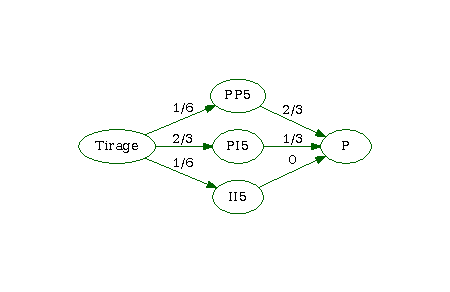
\includegraphics{Cpb01_1.pdf}
 % Cpb01_1.pdf: 0x0 pixel, 0dpi, 0.00x0.00 cm, bb=
 \caption{Exercice \theenumi}
 \label{fig: Cpb01_1}
\end{figure}
